\section{Demonstration}
\author{Mathias}
\subsection{Workflow}
\begin{frame}{Demonstration}
    \framesubtitle{Workflow}
    \begin{itemize}
        \item Start the app on two phones
        \item First a \textbf{server} and then a \textbf{client}
        \item Connect \textbf{client} to \textbf{server}
        \item Select song on \textbf{server}
        \item Listen to \textbf{synchronized} playback
    \end{itemize}
\end{frame}
\begin{frame}{Demonstration}
    \framesubtitle{Workflow --- Connecting Devices}
    \centering
    \begin{tikzpicture}[
        ->,>=stealth',
        auto,
        node distance=3cm,
        thick,
        mock/.style={inner sep=0cm}
        ]

        \node[mock] (mode)
            {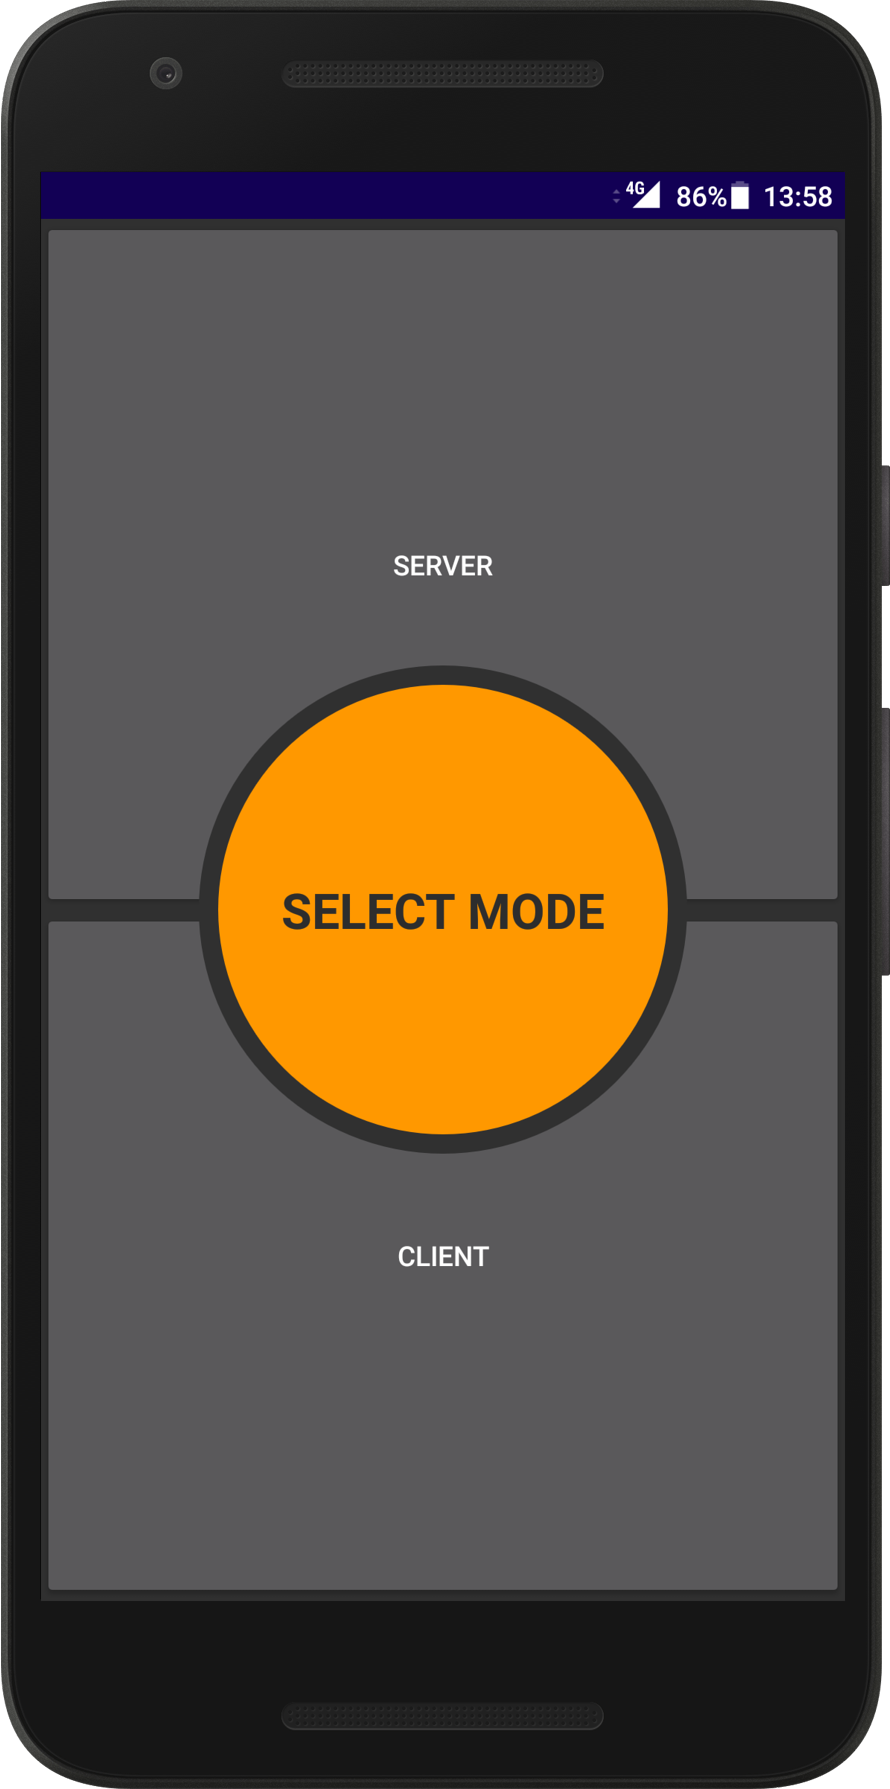
\includegraphics[height=0.35\textheight]{images/ui/mockup/mode_select_nexus5x.png}};
        \node[mock] (server) [above right = -1.3cm and 2cm of mode]
            {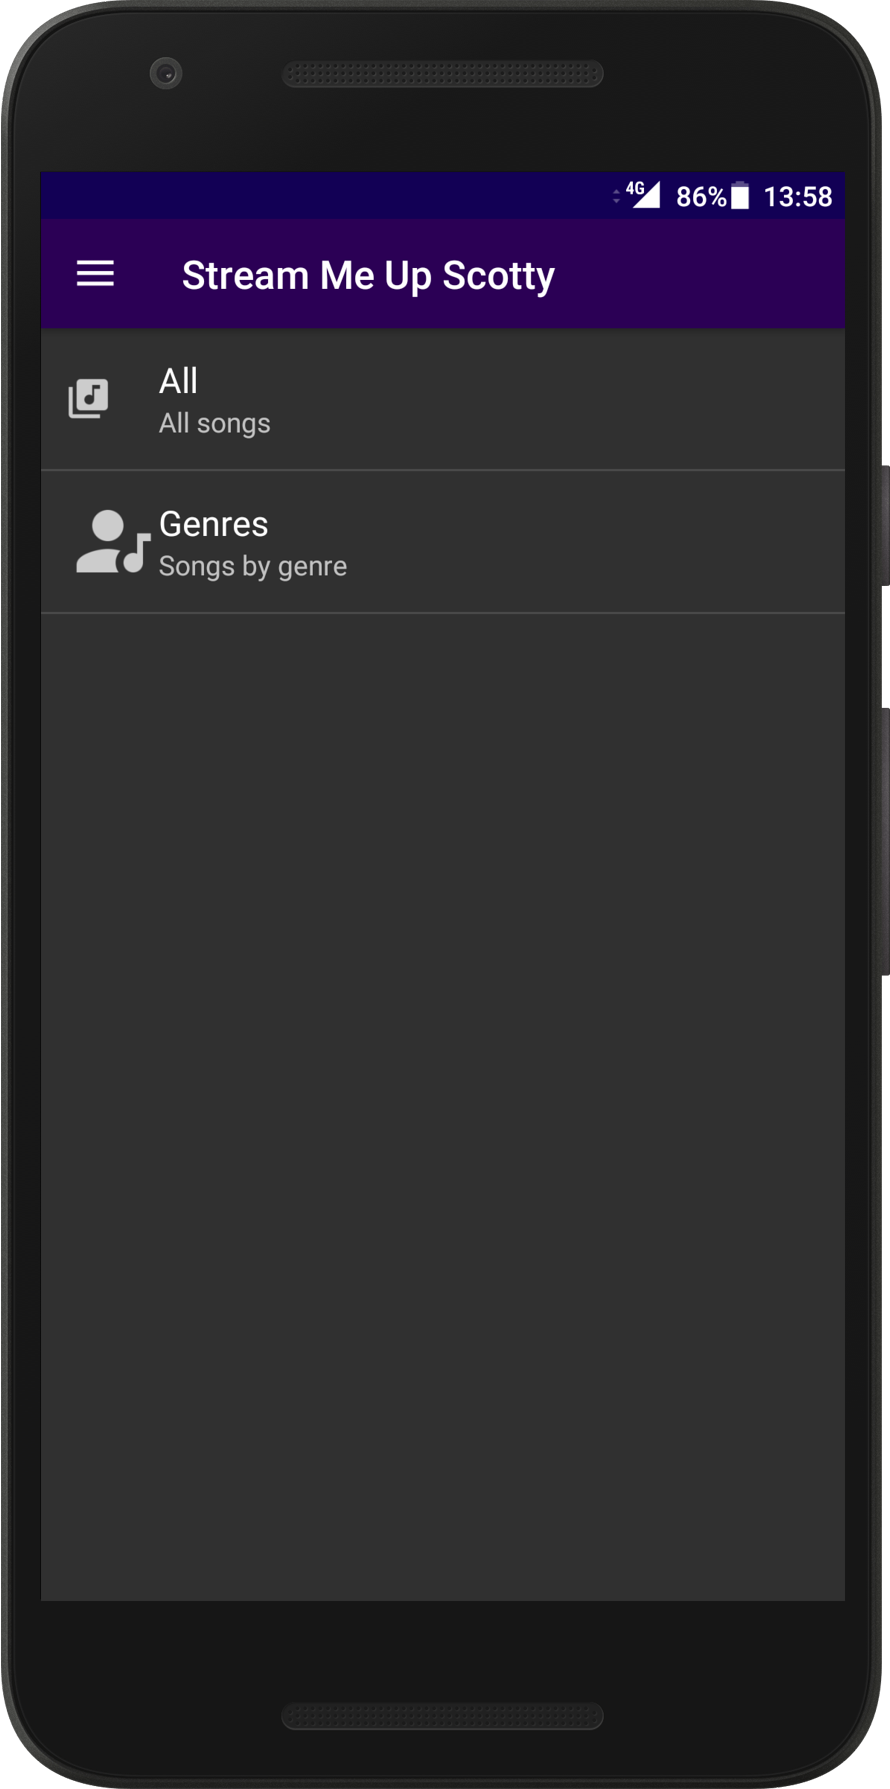
\includegraphics[height=0.35\textheight]{images/ui/mockup/server_1_nexus5x.png}};
        \node[mock] (client) [below right = -1.3cm and 2cm of mode]
            {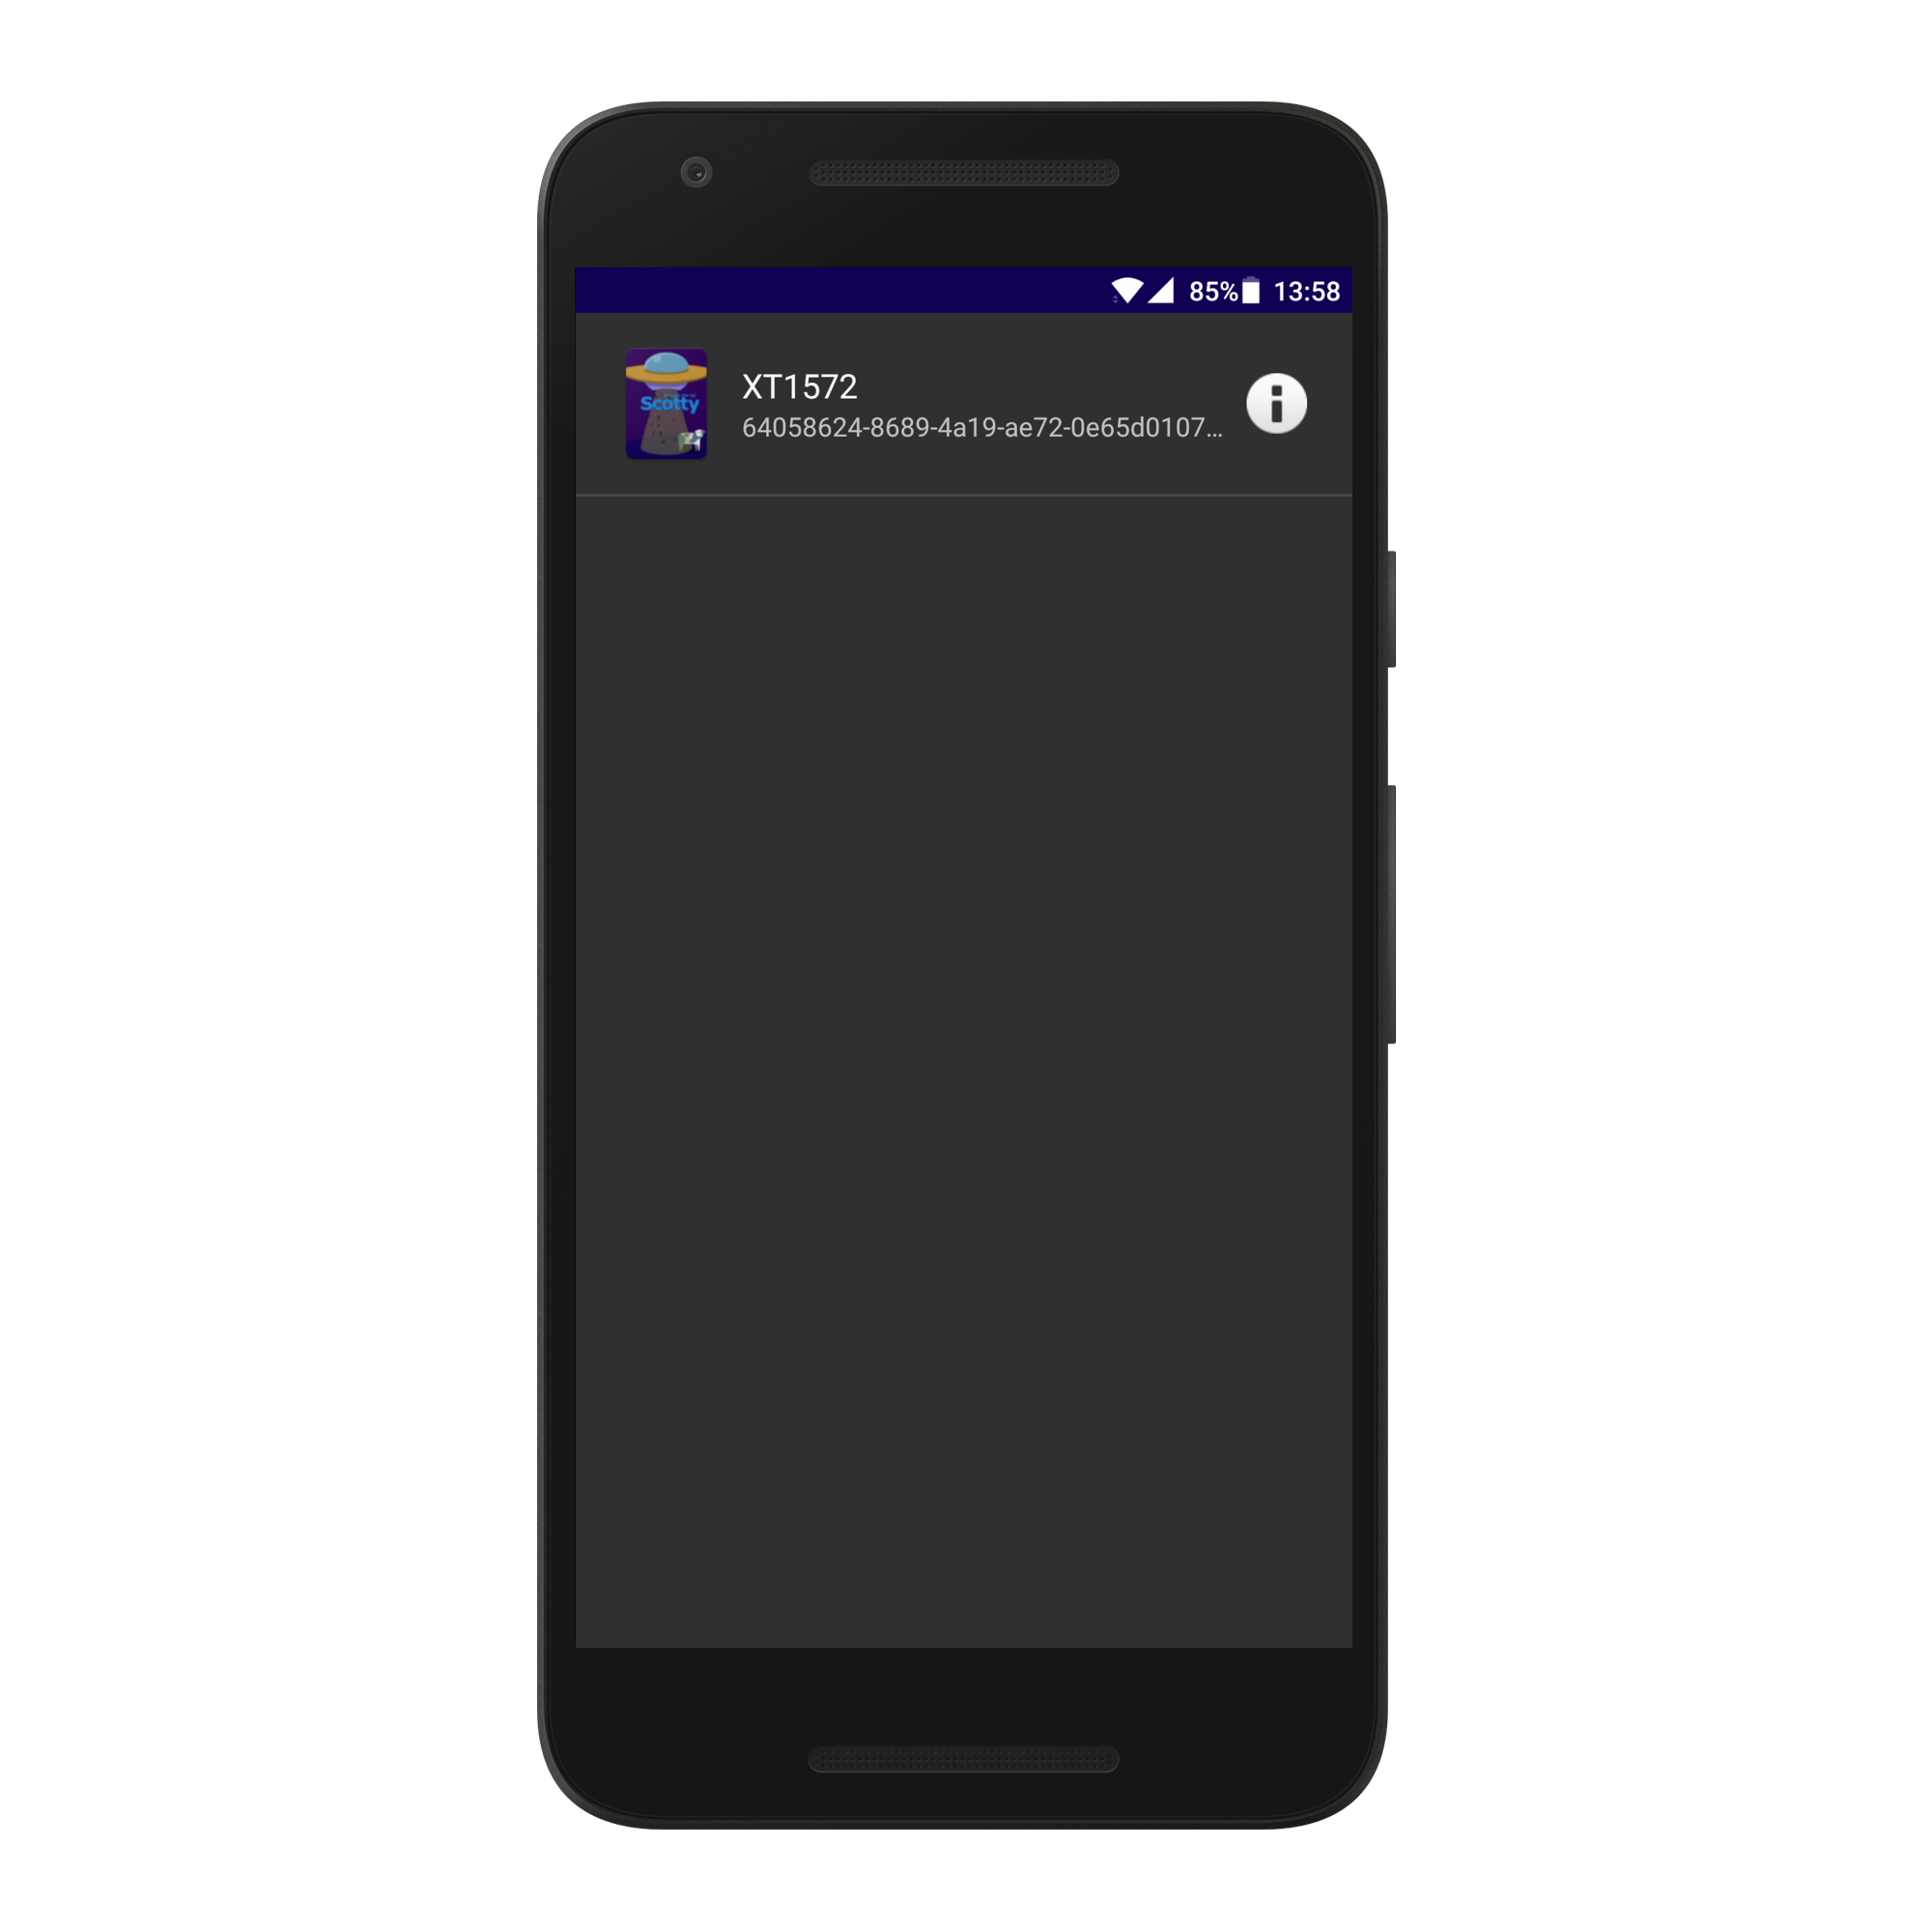
\includegraphics[height=0.35\textheight]{images/ui/mockup/client_join_nexus5x.png}};
        \node[mock] (server_accept) [right = of server]
            {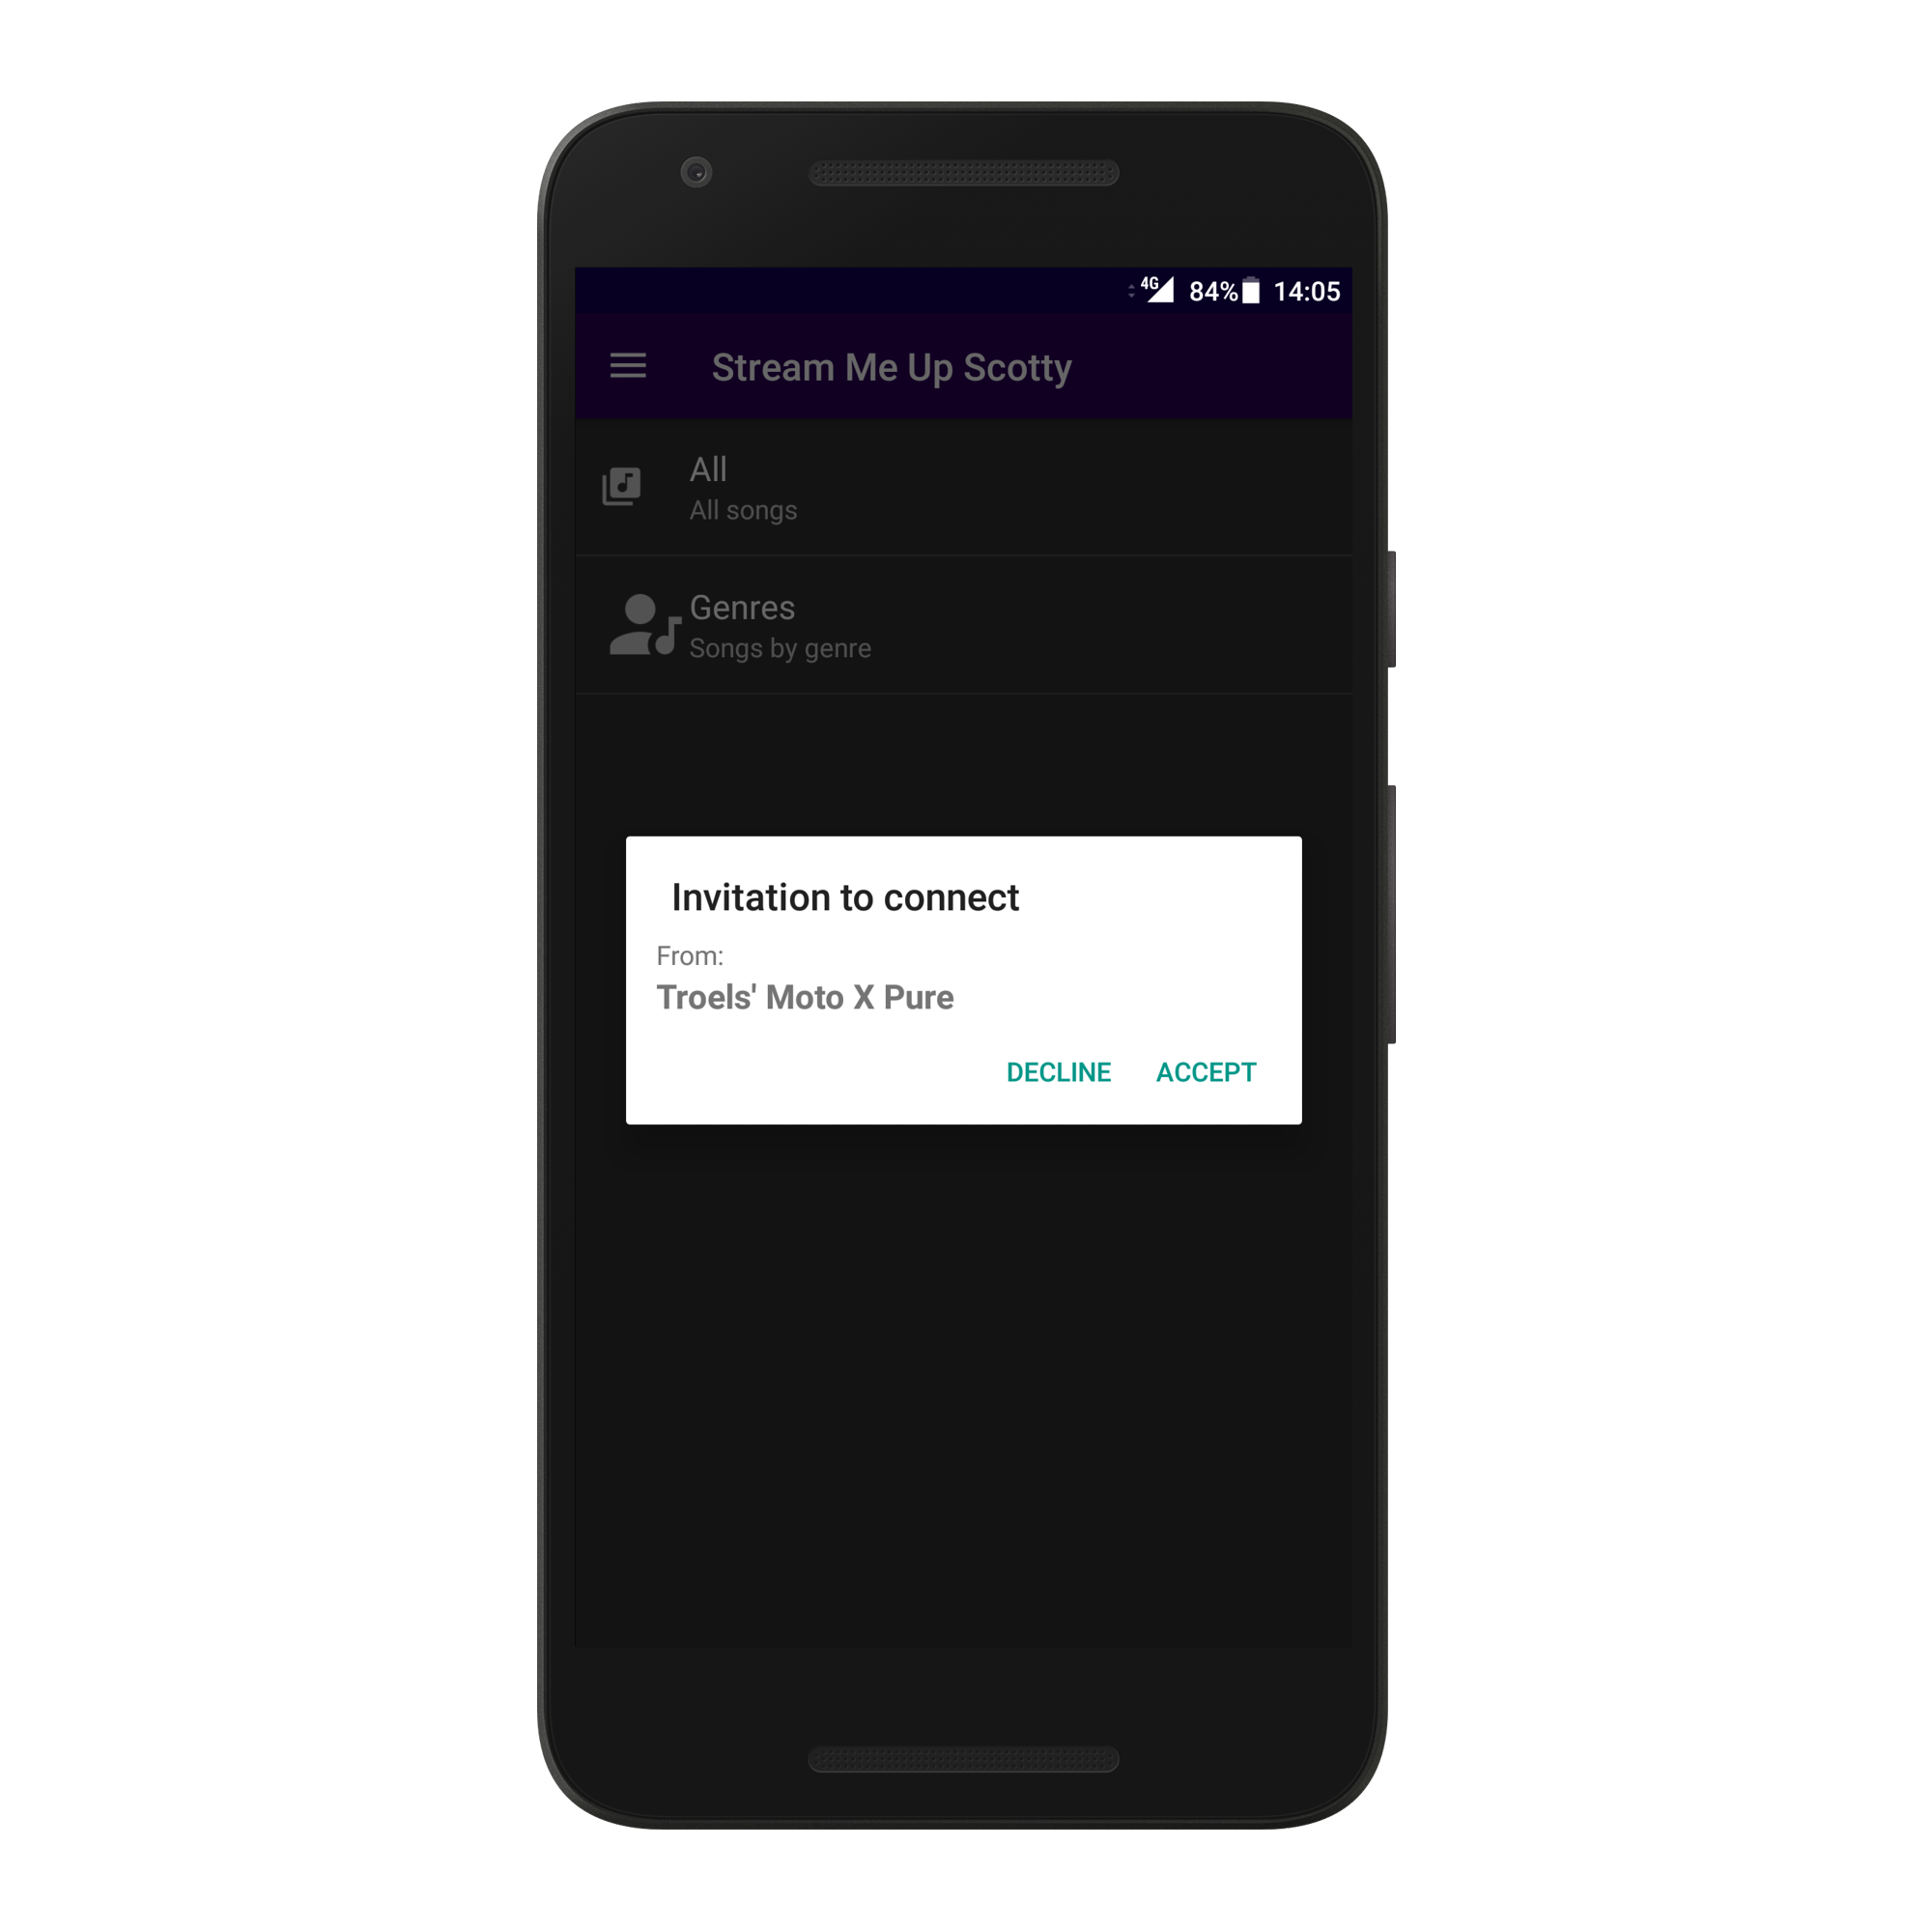
\includegraphics[height=0.35\textheight]{images/ui/mockup/server_accept_nexus5x.png}};
        \node[mock] (client_connected) [right = of client]
            {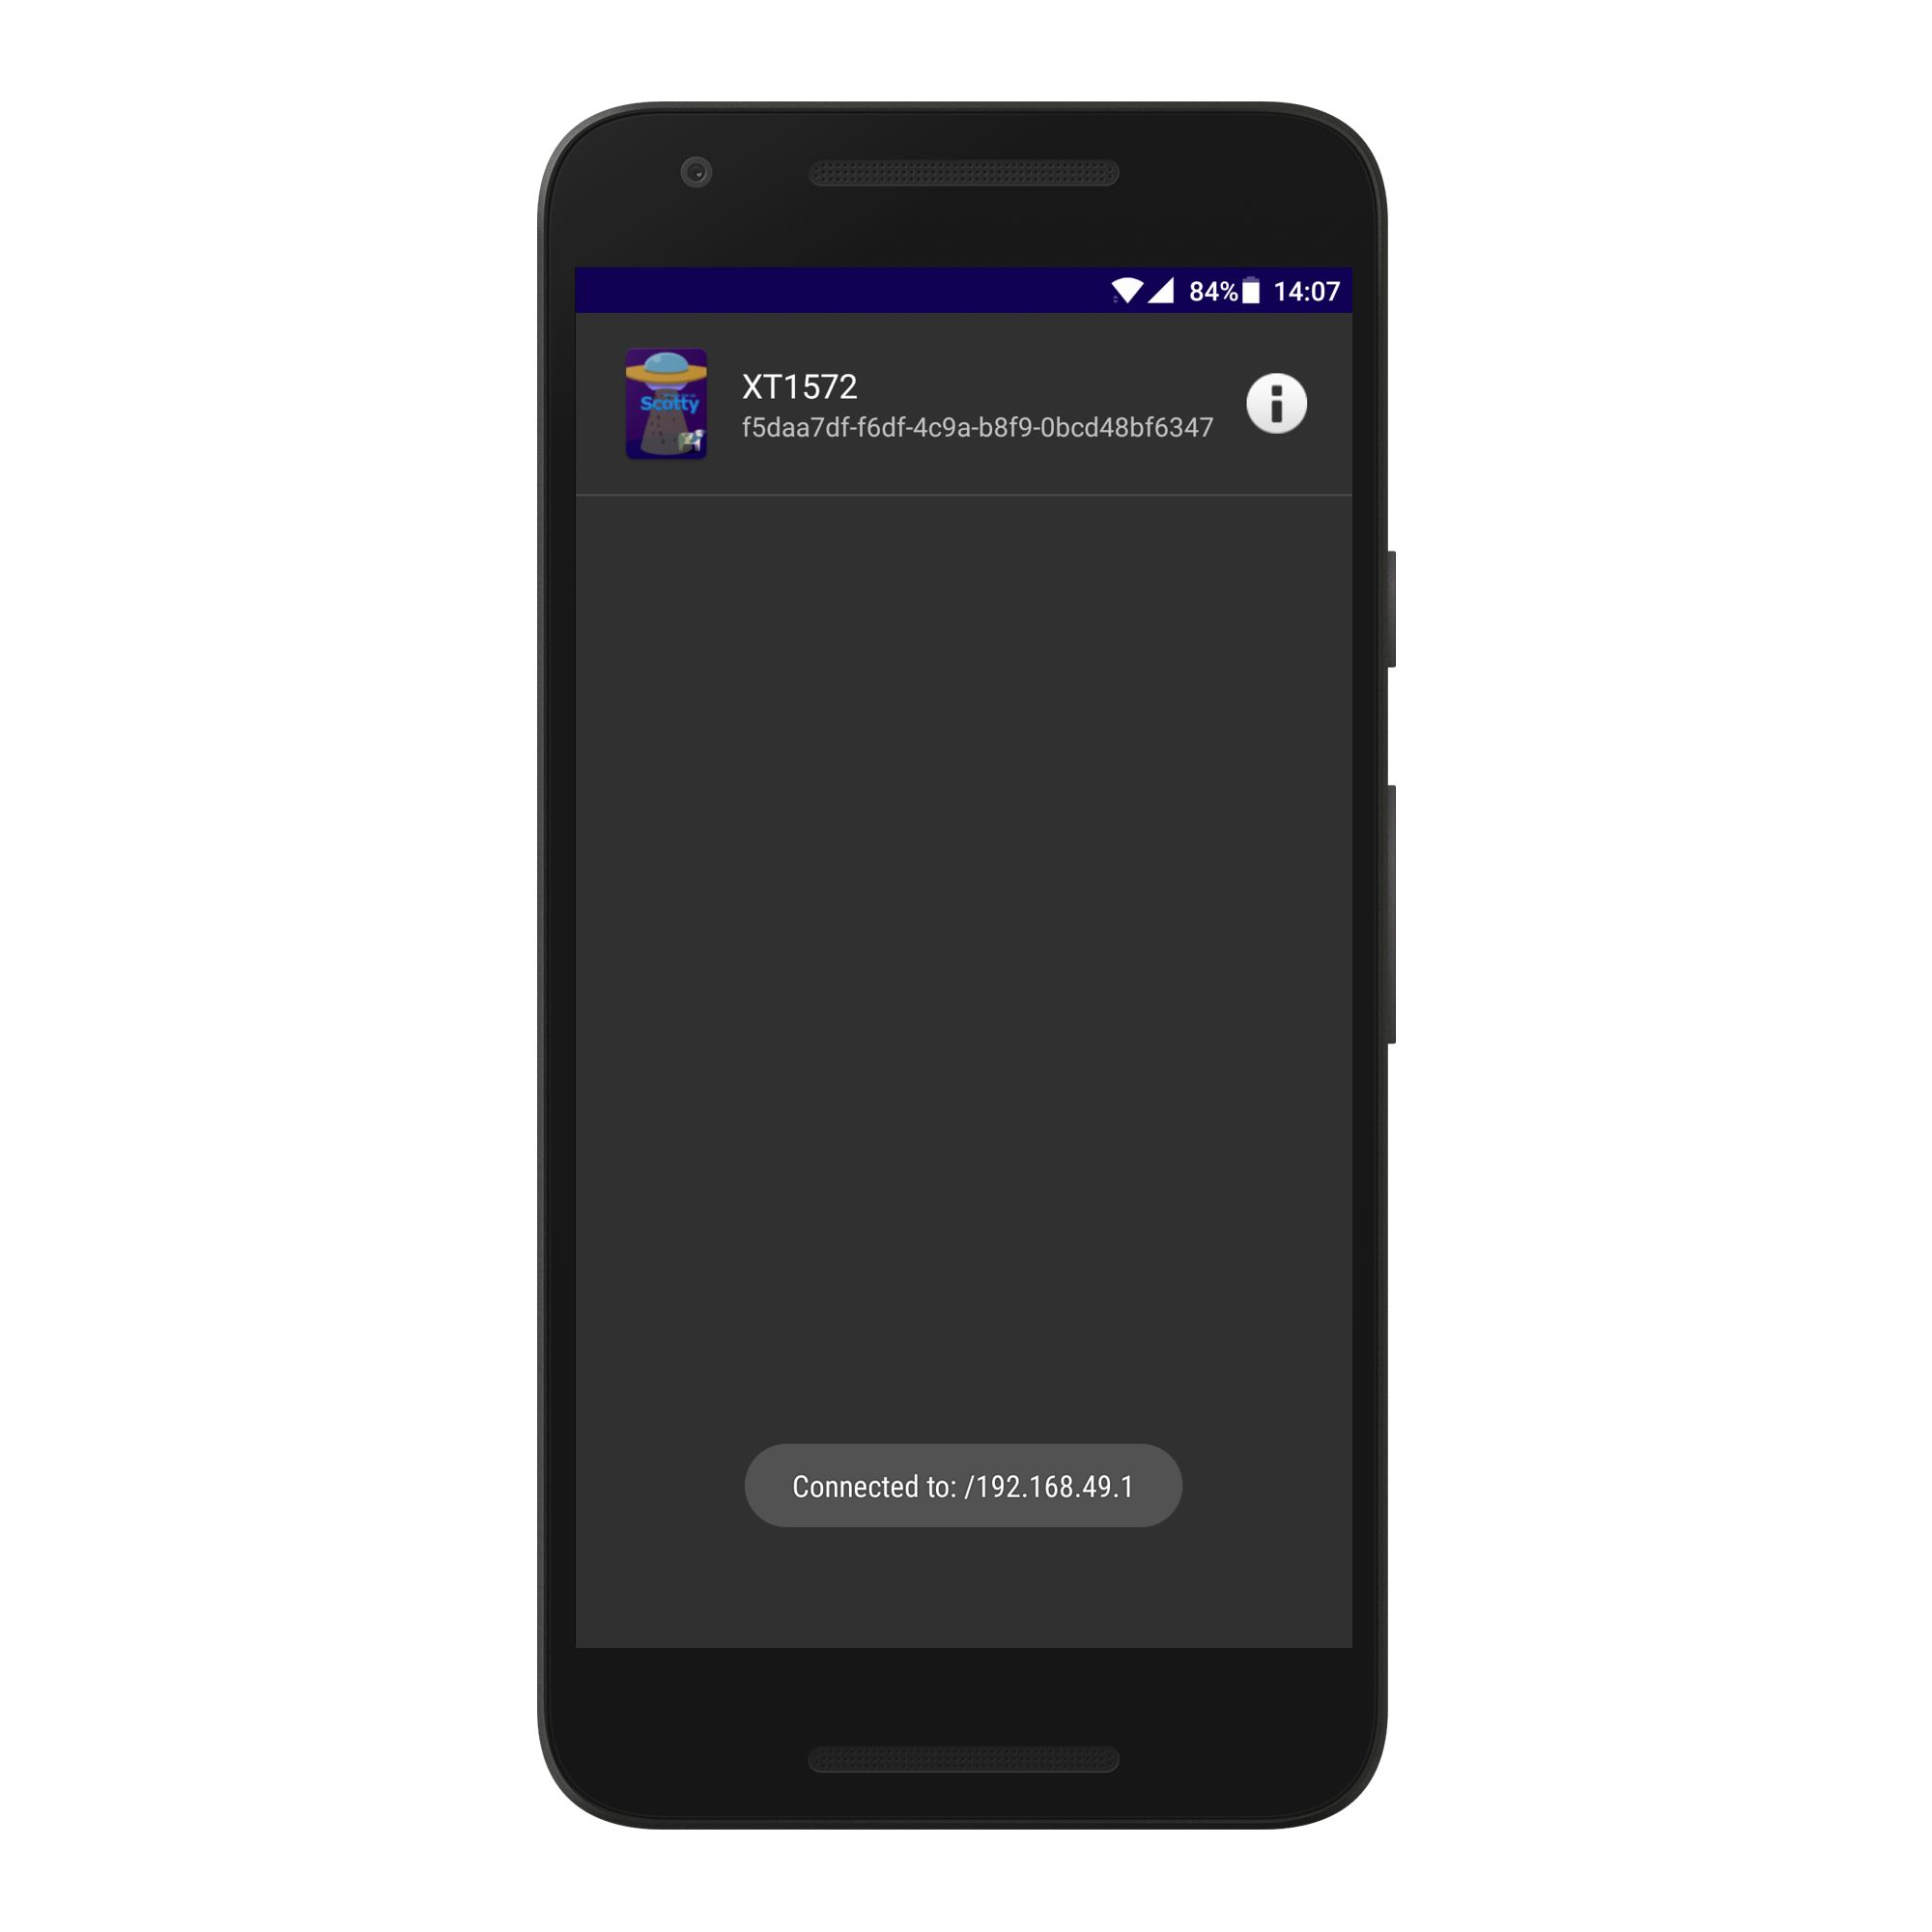
\includegraphics[height=0.35\textheight]{images/ui/mockup/client_connected_nexus5x.png}};

        \draw[->] (mode) -- node [sloped, anchor=center, above] {\tiny Select Server} (server);
        \draw[->] (mode) -- node [sloped, above] {\tiny Select Client} (client);
        \draw[->] (server) -- node [above] {\tiny Get request from client} (server_accept);
        \draw[->] (client) -- node [above] {\tiny Get accept from server} (client_connected);
    \end{tikzpicture}
\end{frame}

\begin{frame}{Demonstration}
    \framesubtitle{Workflow --- Starting Playback}
    \centering
    \begin{tikzpicture}[
        ->,>=stealth',
        auto,
        node distance=4cm,
        thick,
        mock/.style={inner sep=0cm}
        ]

        \node[mock] (media)
            {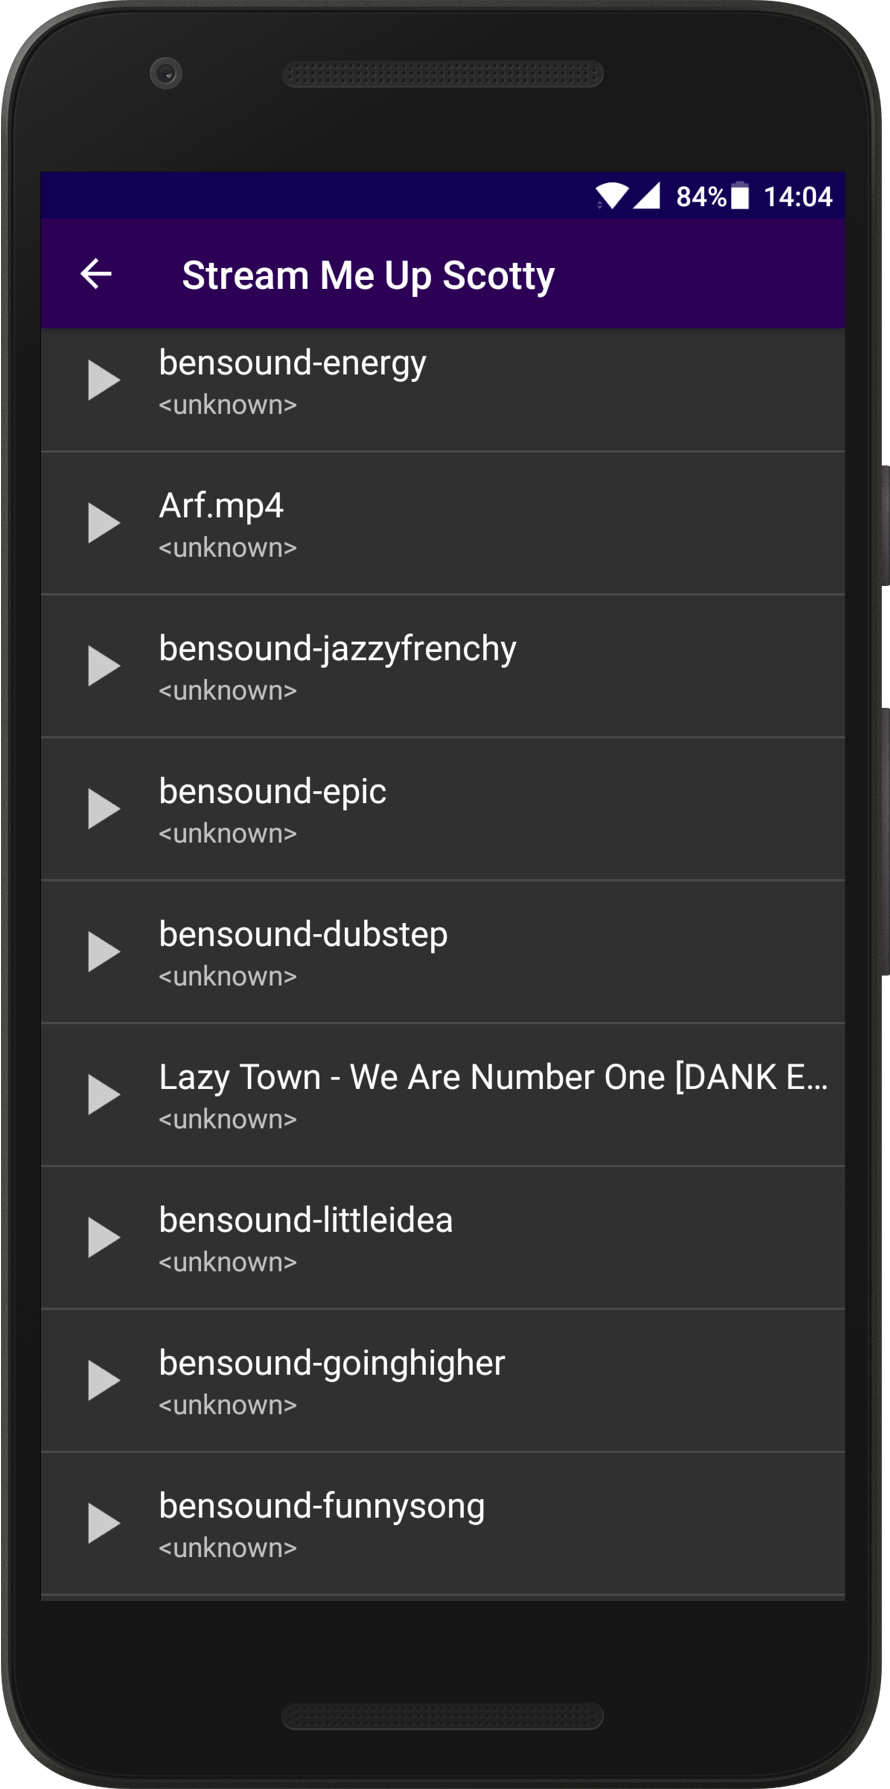
\includegraphics[height=0.35\textheight]{images/ui/mockup/server_media_nexus5x.png}};
        \node[mock] (fullscreen) [right = of media]
            {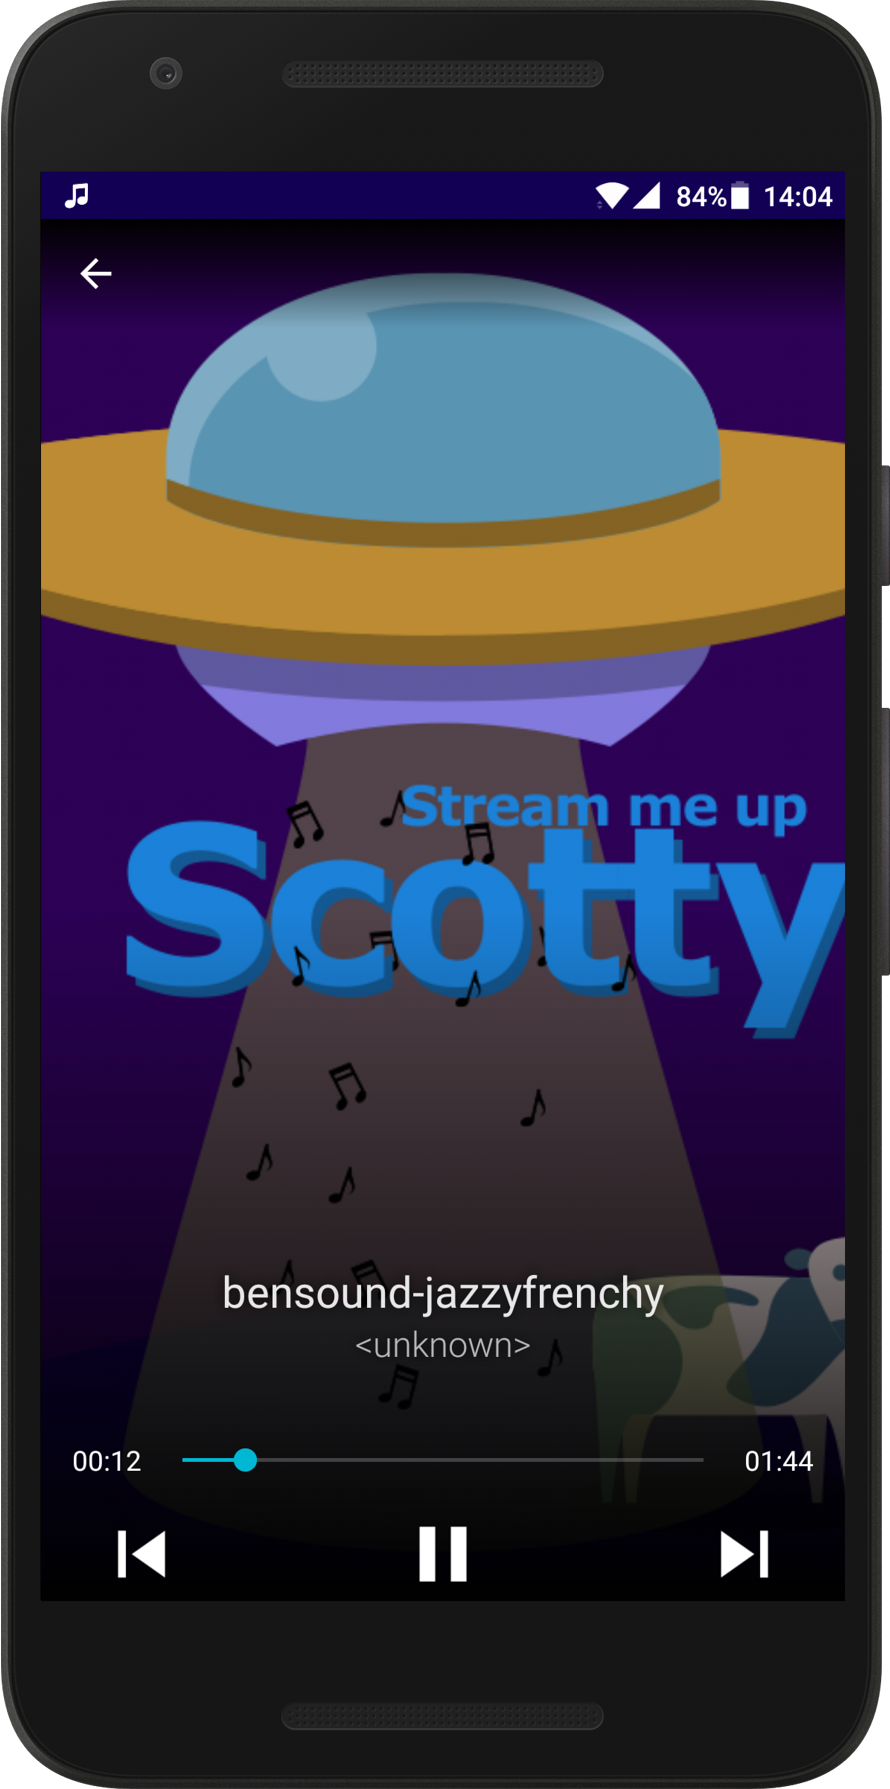
\includegraphics[height=0.35\textheight]{images/ui/mockup/server_player_nexus5x.png}};
        \node[] (splay) [right = 0.3cm of fullscreen] {\Huge$\quarternote$};
        \node[] (splay2) [above right = -0.7cm and 0cm of splay] {\Huge$\twonotes$};
        \node[] (splay3) [below right = -0.4cm and 0cm of splay2] {\Huge$\quarternote$};
        \node[mock] (client) [below = 0.8cm of media]
            {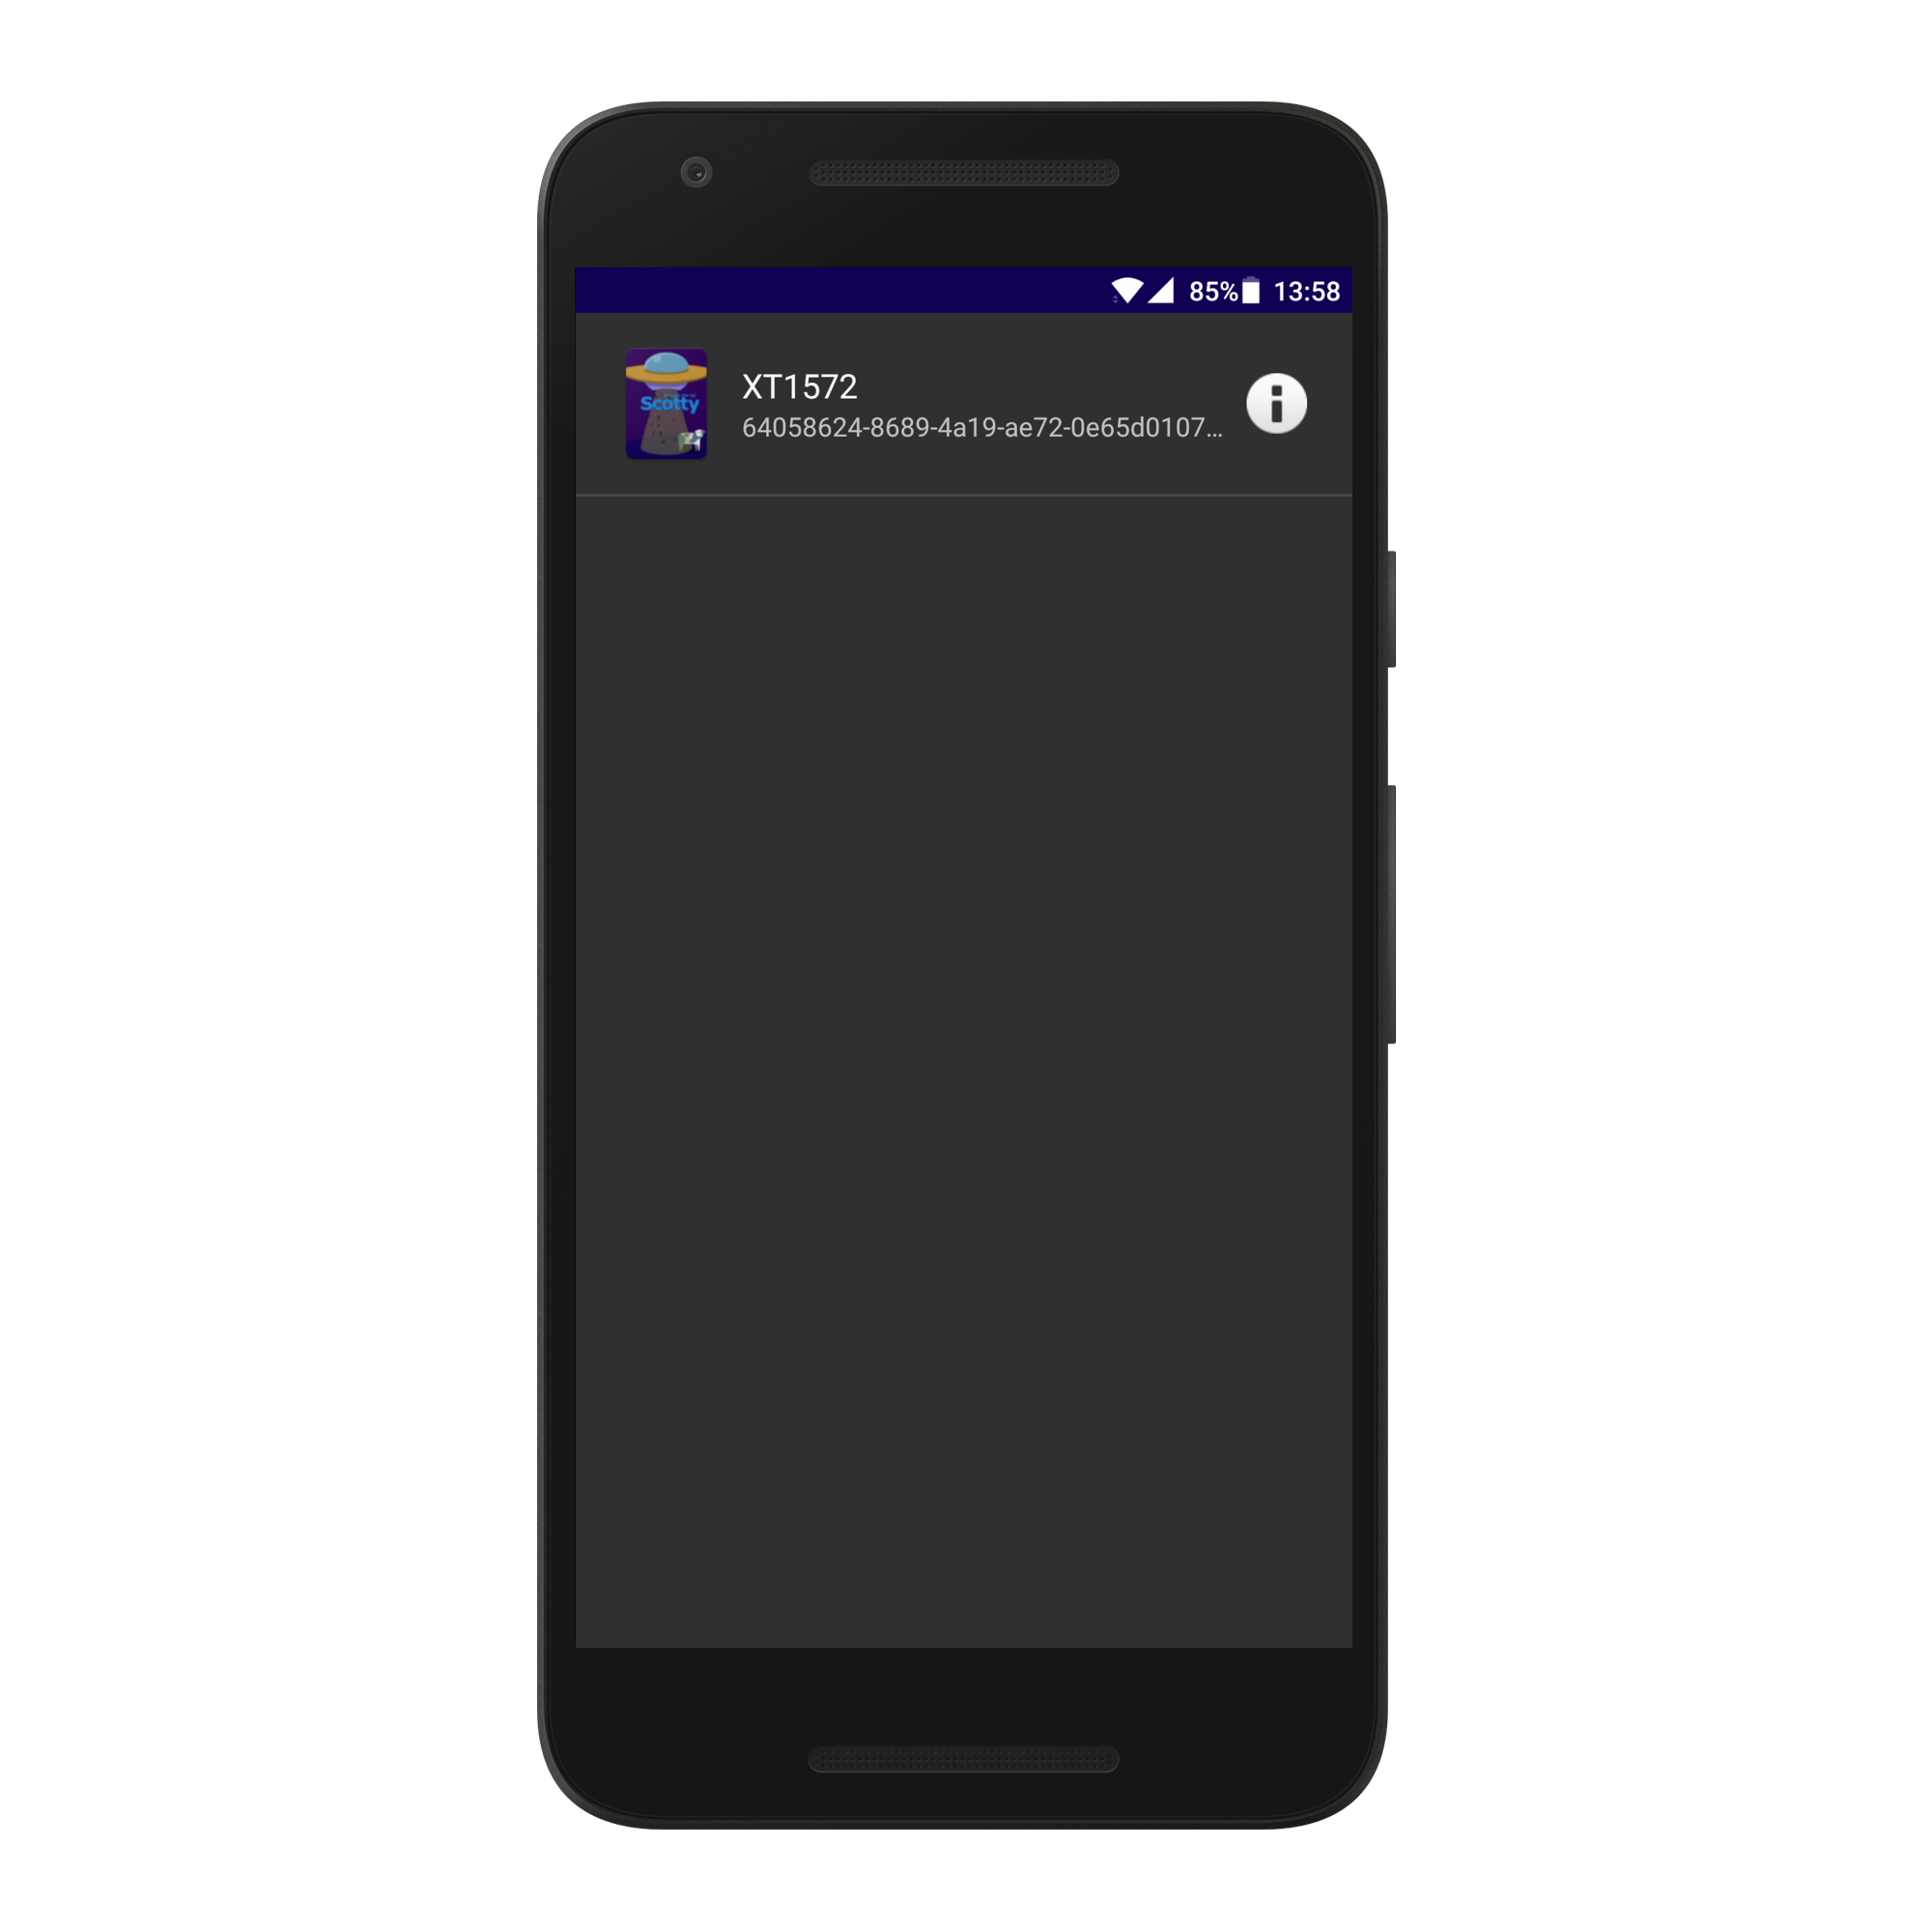
\includegraphics[height=0.35\textheight]{images/ui/mockup/client_join_nexus5x.png}};
        \node[mock] (clientplaying) [right = of client]
            {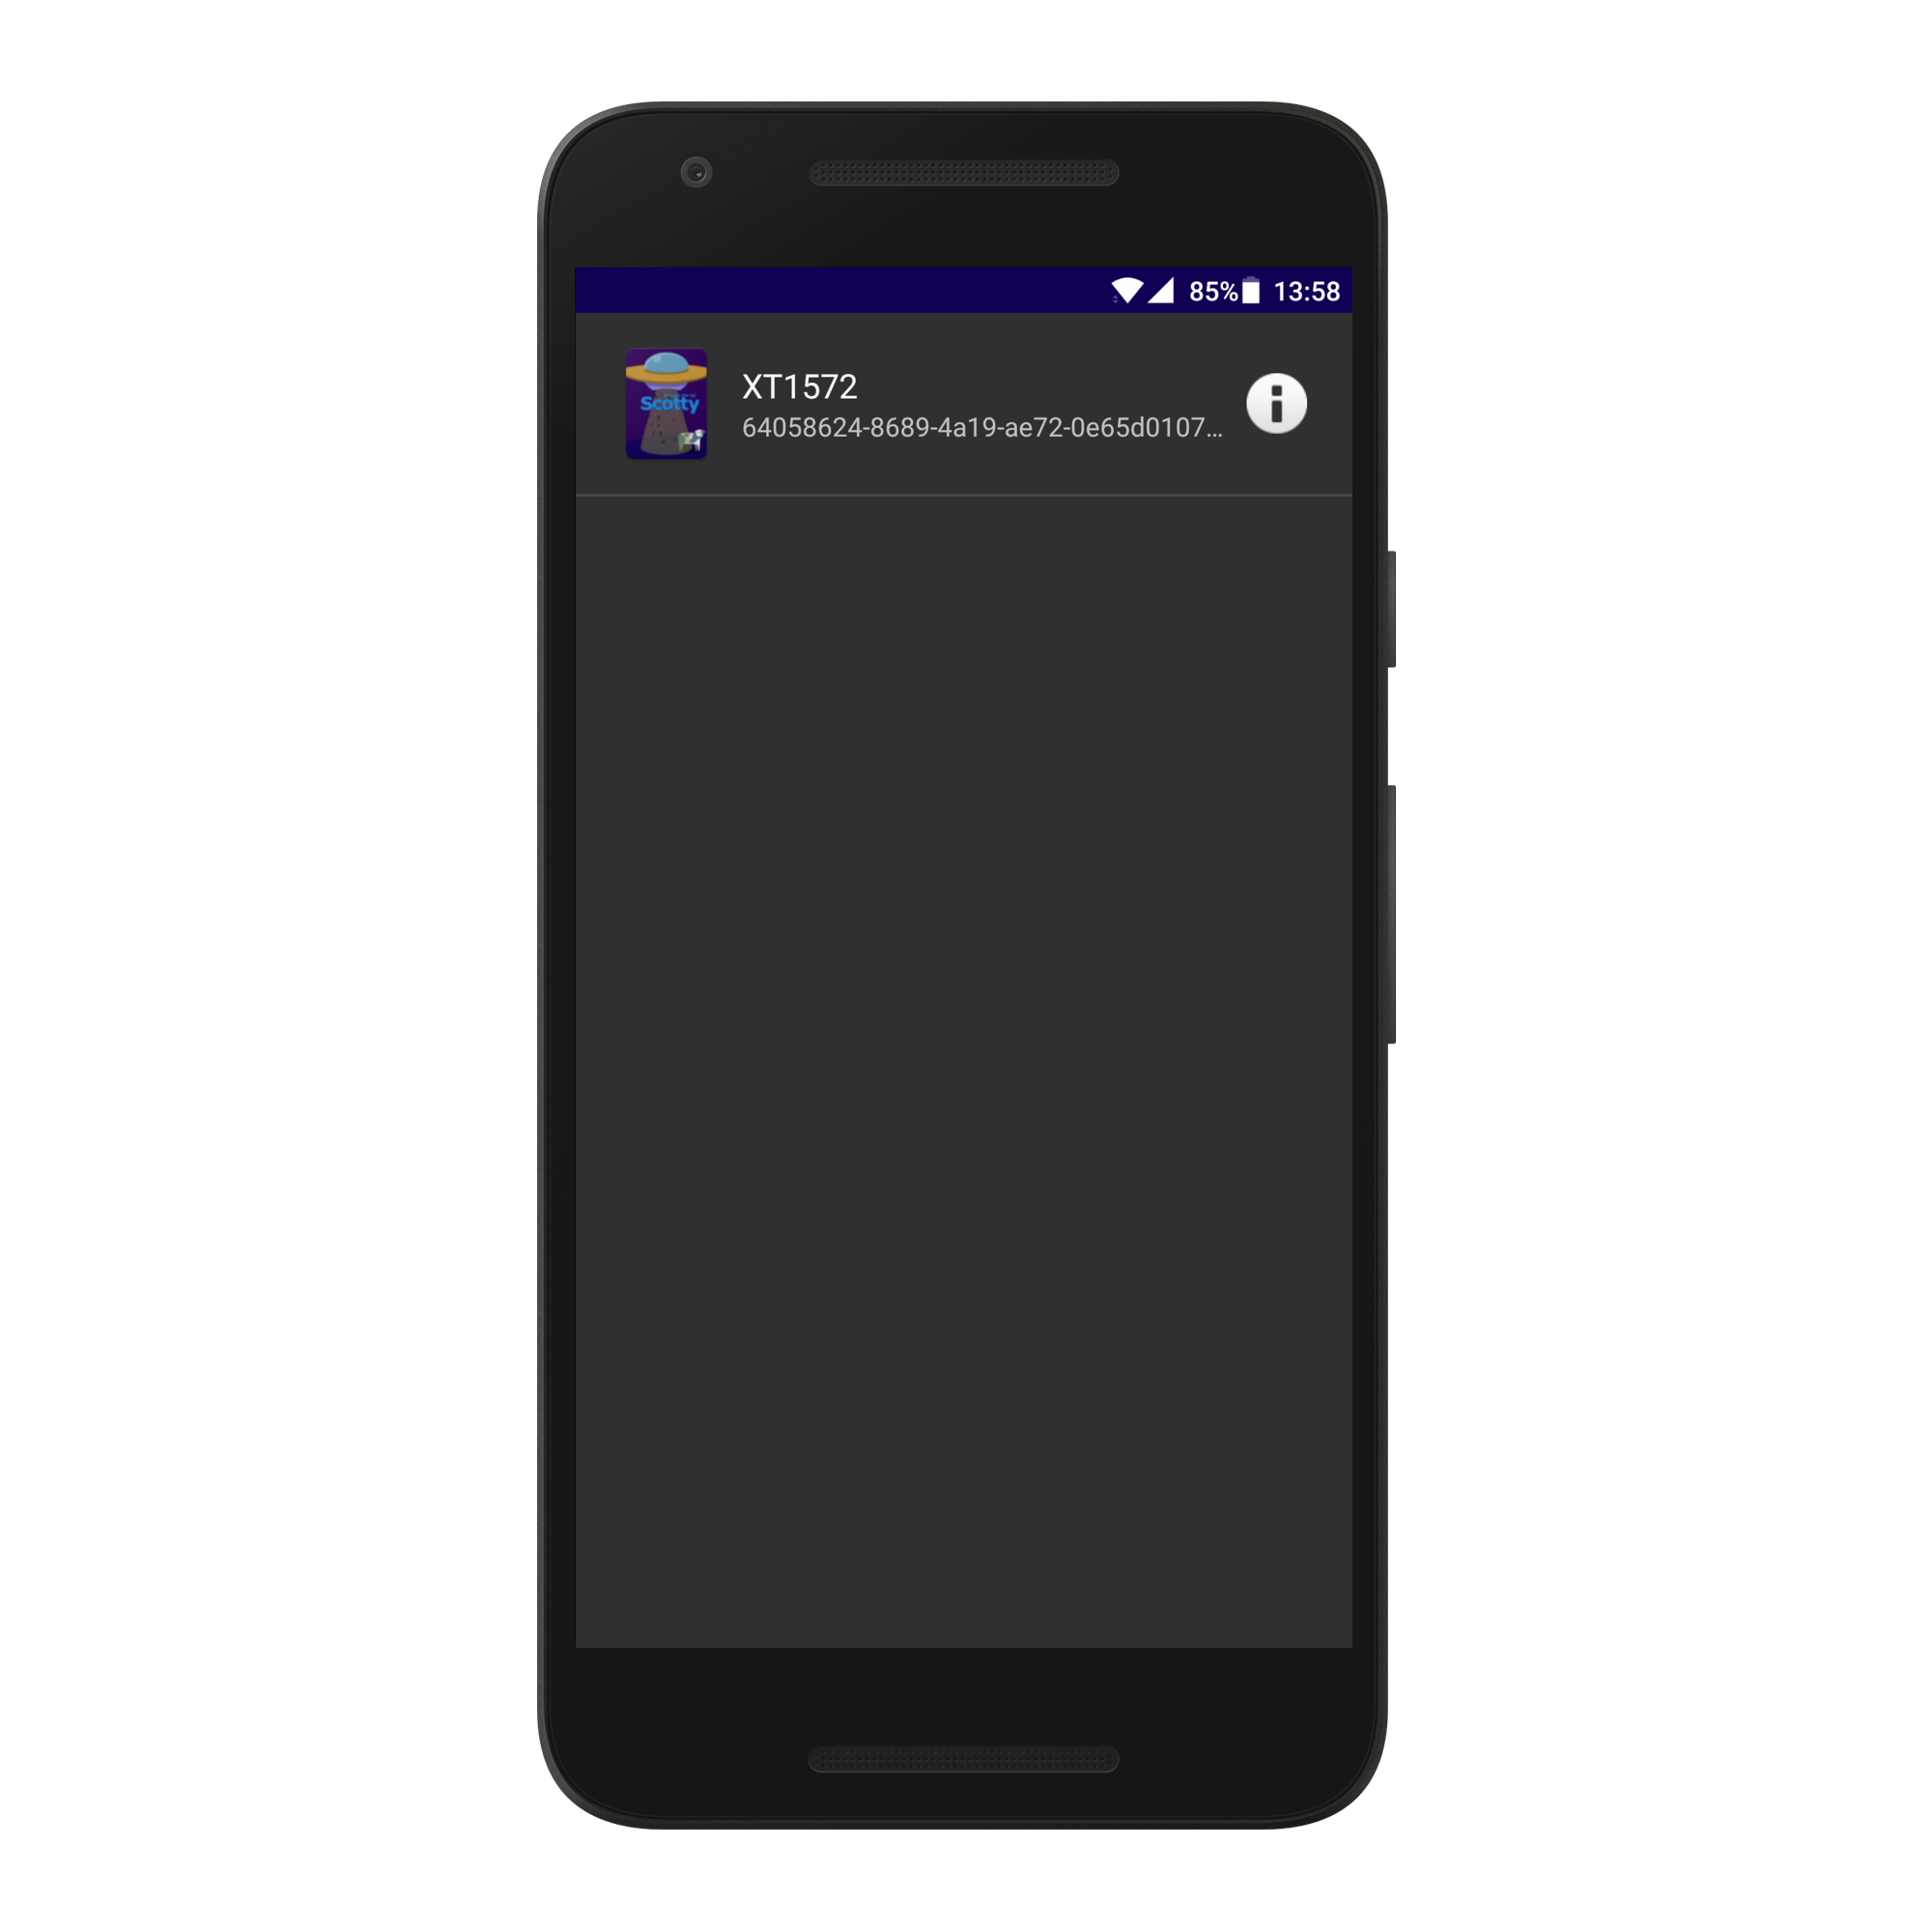
\includegraphics[height=0.35\textheight]{images/ui/mockup/client_join_nexus5x.png}};
        \node[] (cplay) [right = 0.3cm of clientplaying] {\Huge$\quarternote$};
        \node[] (cplay2) [above right = -0.7cm and 0cm of cplay] {\Huge$\twonotes$};
        \node[] (cplay3) [below right = -0.4cm and 0cm of cplay2] {\Huge$\quarternote$};

        \draw[->] (media) -- node [above] {\tiny Choose song and play} (fullscreen);
        \draw[->] (client) -- node [above] {\tiny Receive data and action from server} (clientplaying);
    \end{tikzpicture}
\end{frame}

\subsection{Live Demo}
\begin{frame}{Demonstration}
    \framesubtitle{Live Demo}
    \begin{figure}
    \centering
    
\includegraphics[height=0.7\textheight]{images/scotty_white.png}
    \end{figure}
\end{frame}

\subsection{Inner Workings}

\begin{frame}{Demonstration}
    \framesubtitle{Inner Workings --- Illustration of Audio Buffers and Actions}
    \begin{itemize}
        \item Visualization of how audio is buffered
        \item Useful in debugging
        \item Facilitated by logcat and custom Python script
    \end{itemize}
\end{frame}

\begin{frame}{Demonstration}
    \framesubtitle{Inner Workings --- Static Image}
    \begin{figure}
        \centering
        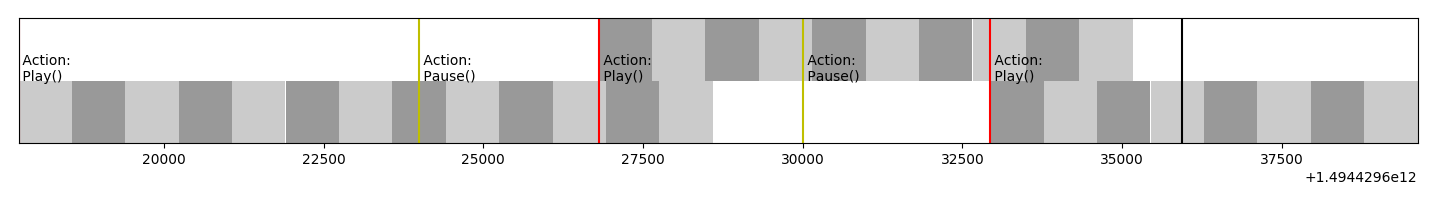
\includegraphics[width=1\textwidth]{images/log_viz_1.png}
    \end{figure}
    \begin{figure}
        \centering
        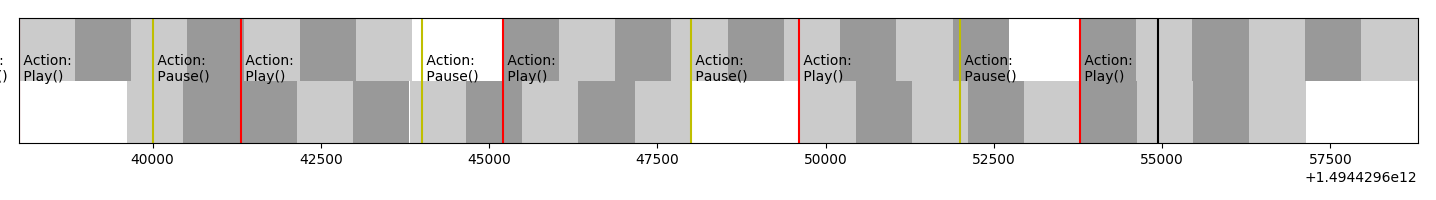
\includegraphics[width=1\textwidth]{images/log_viz_2.png}
    \end{figure}
\end{frame}

\section{Conclusion}

\begin{frame}{Conclusion}
    We have produced an app capable of \textbf{outperforming} the competition in regards to \textbf{audible synchronization}.
    However, it remains \textbf{unpublished} due to missing usability \textbf{polish}.
\end{frame}
